\documentclass{beamer}

\usetheme[secheader]{Boadilla}
\usecolortheme{seahorse}
\usepackage[spanish]{babel} 		% {Con estos dos anda
\usepackage[utf8]{inputenc} 		% todo lo que es tildes y ñ}
\usepackage{graphicx}

\title{Pedí un taxi ahora con: TAXINOW}
\author{Martín Carreiro - Pablo Rago - Juan Manuel Tastzian}
\date{2 de Julio de 2014}
\institute[2014]{Facultad de Ciencias Exactas y Naturales}

\begin{document}

\frame{\titlepage}

\section{Sobre TaxiNow}

\frame {
	\frametitle{¿Qué es TaxiNow?}
	TaxiNow es una aplicación de dos enfoques
	\begin{itemize}
		\item<2-> Enfoque de taxista.
		\item<3-> Enfoque de pasajero de un taxi.
	\end{itemize}
}

\frame {
	\frametitle{¿Qué es TaxiNow?}
	Elección de enfoque:
	\begin{center}
		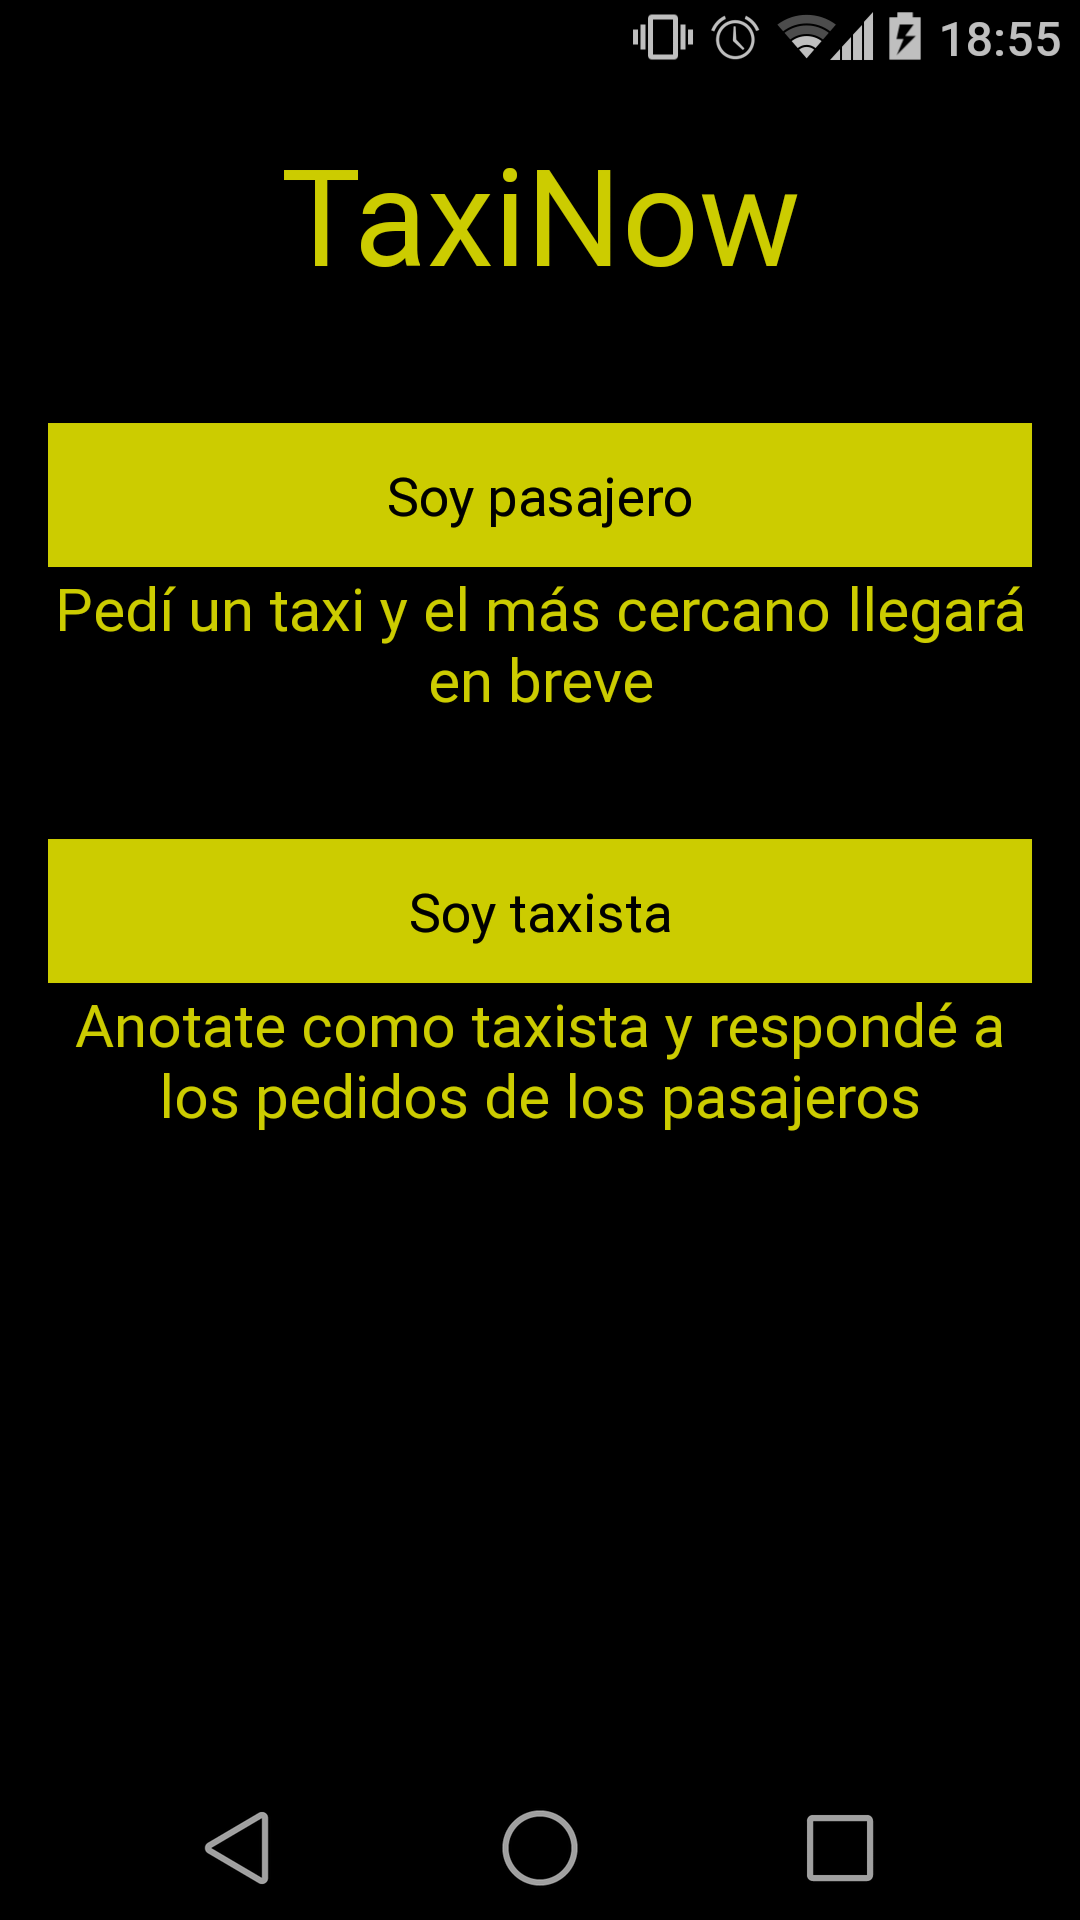
\includegraphics[scale=0.1]{./screenshots/01_UserTypeChoosing.png}	
	\end{center}
}

\frame {
	\frametitle{¿Qué es TaxiNow?}
	Un taxista puede:
	\begin{itemize}
		\item <2-> Registrarse en la aplicación.
		\item <3-> Completar su perfil.
			\begin{itemize}
				\item <4-> Publicar una foto de su vehículo.
				\item <5-> Registrar su marca, modelo y patente del taxi.
			\end{itemize}
		\item <6-> Esperar que lleguen viajes.
		\item <7-> Aceptar o ignorar viajes.
	\end{itemize}
}

\frame {
	\frametitle{Enfoque de taxista}
	\begin{center}
		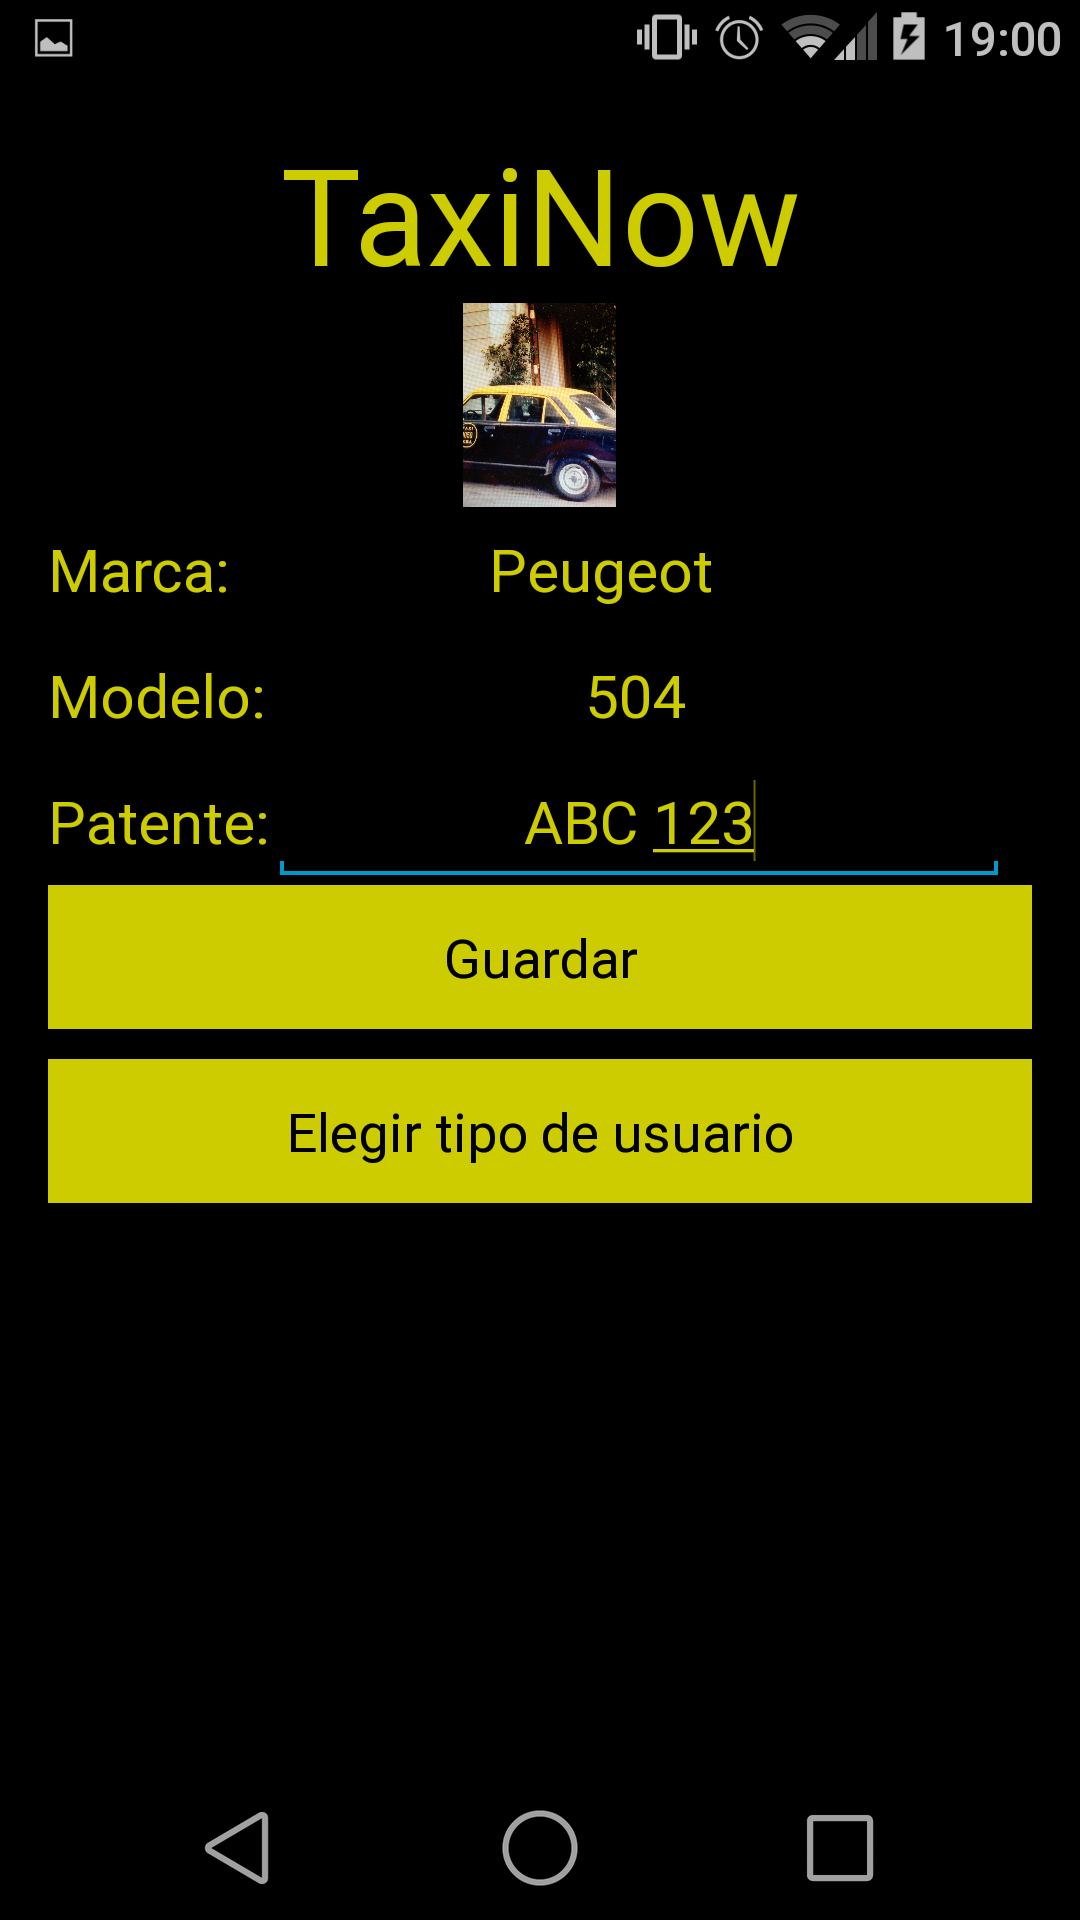
\includegraphics[scale=0.1]{./screenshots/06_TaxiConfigCompleta.png}	
	\end{center}
}

\frame {
	\frametitle{¿Qué es TaxiNow?}
	Un pasajero puede:
	\begin{itemize}
		\item <2-> Registrarse en la aplicación.
		\item <3-> Decir a donde quiere ir y pedir un taxi.
	\end{itemize}
}

\frame {
	\frametitle{Enfoque de taxista}
	\begin{center}
		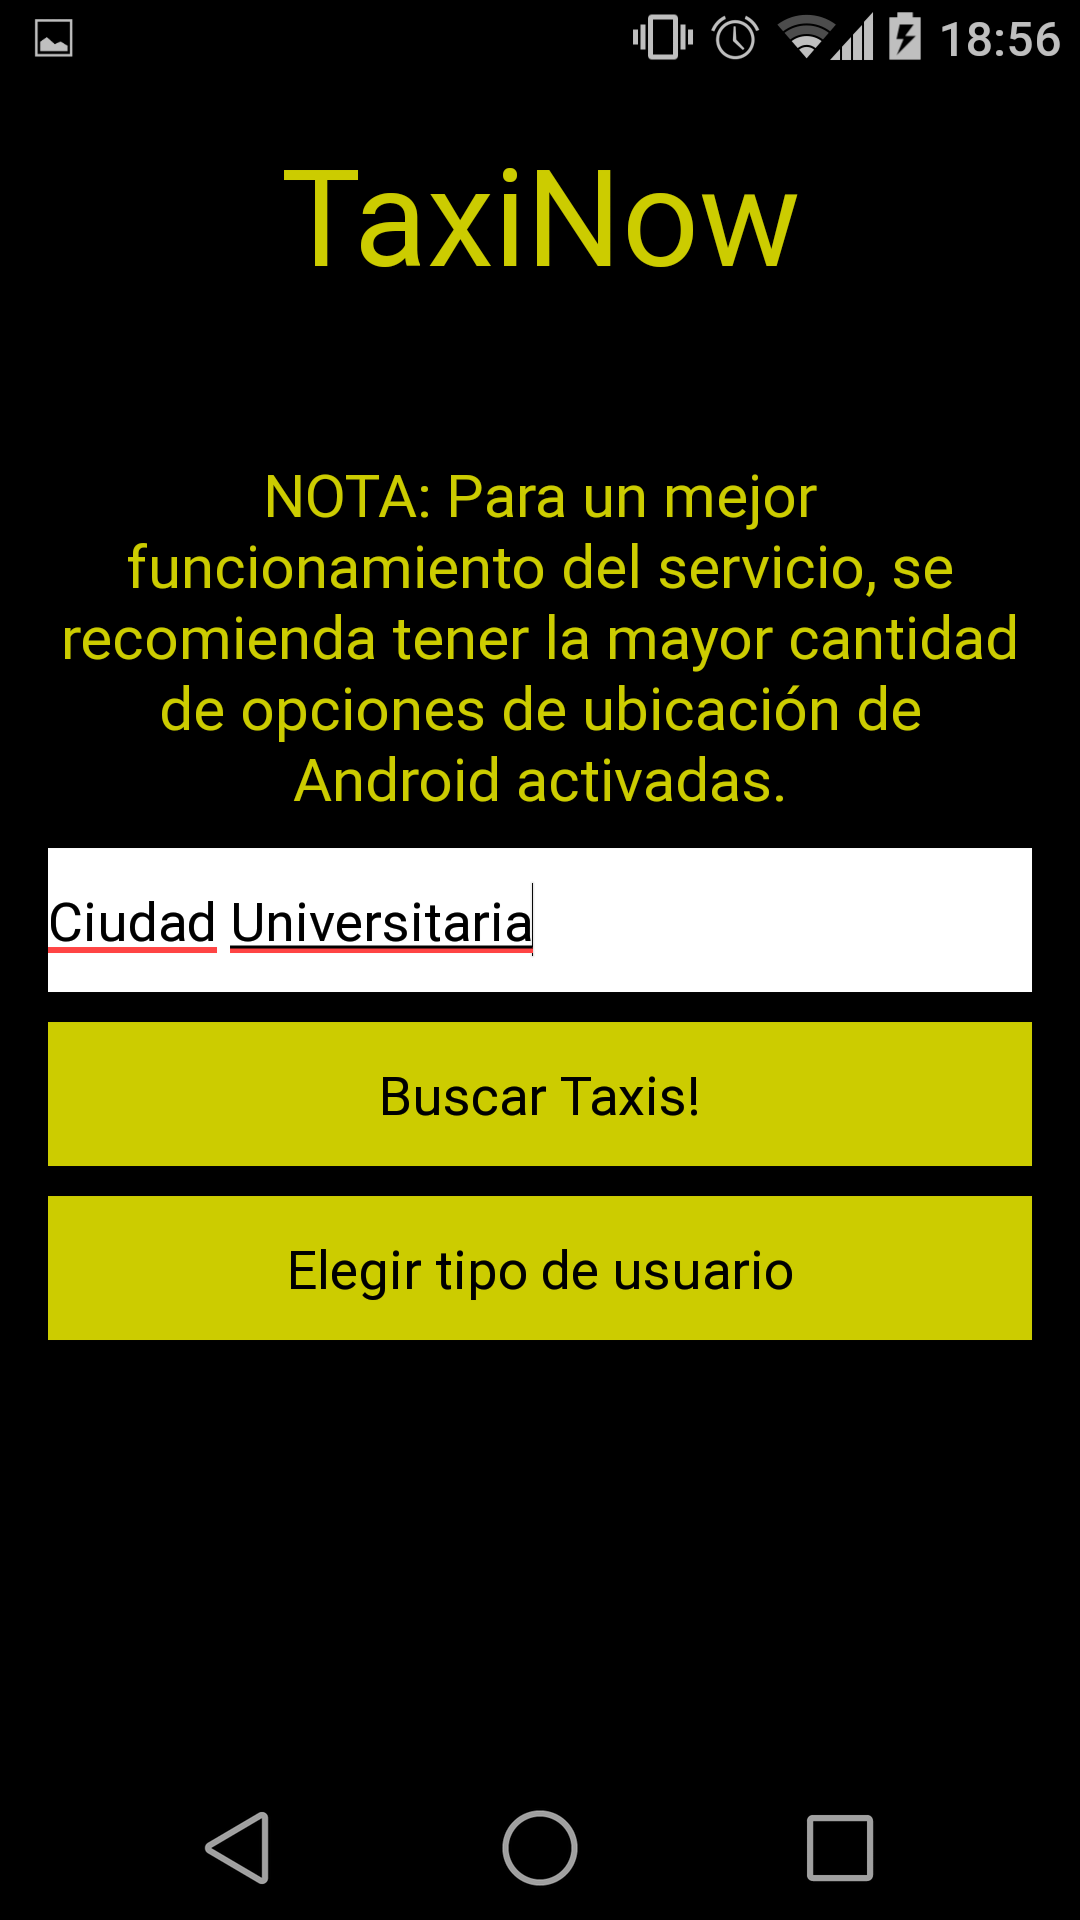
\includegraphics[scale=0.1]{./screenshots/03_PassengerCompleta.png}	
	\end{center}
}

\frame {
	\frametitle{OJO QUE ACA ARRANCAN FRAMES VIEJOS}
	BORRAR DE ACÁ EN ADELANTE, LO DEJÉ COMO PRUEBA
}



\frame {
	\frametitle{¿Cuánto les duraba la batería del Nokia 1100 y similares?}
	\begin{itemize}
		\item<2-> ¿15 hs?
		\item<3-> ¿2 días?
		\item<4-> Como 4 o 5, tranqui!
	\end{itemize}
}

\frame{
	\frametitle{Eso ya no pasa con los Smartphones}
	\begin{itemize}
		\item[] <2-> Lamentablemente, todas las ventajas mencionadas antes necesitan mucha energía para funcionar.
		\item[] <3-> Y por eso, la batería de nuestros celulares de hoy dura entre 12 y 16 horas, promedio, siendo unas 18 o 20 horas una excelente duración de batería (ni hablar de más tiempo).
	\end{itemize}
}

\section{Manejo de energía en Android}

%\subsection{Wakelock API}

\frame {
	\frametitle{Manejo de energía en Android}
	\begin{itemize}
		\item[] <1-> ¿Cómo maneja la energía Android?
		\begin{itemize}
			\item<2-> De manera \textbf{agresiva}.
		\end{itemize}
		\item[] <3-> ¿Le pega para que se porte bien?
		\begin{itemize}
			\item<4-> No \textbf{tan} agresiva, pero le corta el chorro a todo en el momento \textbf{inmediato} en el que se deja de usar.
		\end{itemize}
	\end{itemize}
}

\frame {
	\frametitle{Manejo de energía en Android}
	\begin{itemize}
		\item[] <1-> Pero, ¿y si, como desarrollador, quiero tener el procesador corriendo para recibir algún update o notificación?
		\begin{itemize}
			\item<2-> Ahí es donde entra en juego la \textbf{Wakelock API}.		
		\end{itemize}
	\end{itemize}
}

\frame {
	\frametitle {Manejo de energía en Android}
	\begin{itemize}
		\item[] <1-> Lamentablemente, la complejidad del sistema operativo y los errores que pueden cometer los desarrolladores hacen que el uso inapropiado de Wakelocks se manifiesten como \textit{no-sleep-bugs}.
		\item[] <2-> Los autores del paper decidieron intentar mitigar el problema implementando una herramienta que verifica la ausencia de estos bugs con respecto a una serie de políticas específicas sobre los Wakelocks, utilizando un framework de flujo de datos para analizar las aplicaciones.
		\item[] <3-> Pero...
		\item[] <4-> ¿qué es la Wakelock API?
	\end{itemize}
}

\frame {
	\frametitle {Wakelock API}
	\begin{itemize}
		\item <2-> Permite a los desarrolladores dar directivas específicas sobre los recursos al sistema operativo, ya que Android pone todo en sleep mode ni bien se ponen en estado idle (reposo).
		\item <3-> Es una forma de decir ``esto no me lo apagues" (GPS, pantalla, CPU, etc.).
		\item <4-> Entonces si necesito que algo en particular esté encendido en un momento crítico, pido un Wakelock sobre el mismo para que no se apague, lo uso, y cuando termino, lo libero.
		\item <5-> Genial! Pero ¿qué pasa si me olvido de liberarlo?
		\item <6-> Buena pregunta... ¿cuánto se acuerdan de Orga 2?
	\end{itemize}
}

\frame {
	\frametitle {Repaso de Orga 2}
	\begin{itemize}
		\item <2-> En Orga 2 me enseñaron que debo hacer un free por cada malloc...
			\begin{itemize}
				\item <3-> ...sino \tiny me pegaban.
			\end{itemize}
		\item <4-> Hablando en serio: si no liberan el Wakelock, pasa lo que esperan.
		\item <5-> El recurso no se libera, queda activo, y se \textbf{gasta batería} innecesariamente.
		\item <6-> Esto es a lo que en el paper se lo llama \textit{no-sleep bug}.
		\item <7-> Vendría a ser la versión de ``power management" de los ``memory leaks".
	\end{itemize}
}

%{
%	This text will stay on all pages.
%	\only<1>{
%		\begin{itemize}
%			\item<1->This will only appear on the first page
%			\item<1->This is also only for the first page
%		\end{itemize}
%	}
%	\only<2>{
%		\begin{itemize}
%			\item<2->This will only appear on the second page
%		\item<2->This is also only for the second page
%		\end{itemize}
%      }
%}
%
\section{Planteo del paper}

\frame {
	\frametitle{Planteo del paper}
	\begin{itemize}
		\item[] <2-> Los autores del paper desarrollaron una herramienta que permite verificar la ausencia de estos bugs con respecto a una serie de \textbf{políticas específicas sobre los Wakelocks}, utilizando un framework de flujo de datos para analizar las aplicaciones.
		\item[] <3-> Lo peor de todo esto, es que estos bugs son \text{muy difíciles de detectar}, ya que no hace que la app funcione mal o crashee, sino que te reduce la duración de batería del equipo, pasando casi desapercibida como causante de dicho problema.
		\item[] <4-> Pero para entender todo esto, primero hay que entender un poco como funciona el sistema operativo Android por detrás.
	\end{itemize}
}

\frame{
	\frametitle{Un poco de contexto}	
	\begin{itemize}
		\item[] <1-> \textbf{Manejo de energía}
			\begin{itemize}
				\item <2-> Creación, adquisición y liberación de objetos \textbf{Wakelock}.
				\item <3-> Asociados a un recurso particular (CPU, pantalla, GPS, etc.).
				\item <4-> En manos del desarrolador.
			\end{itemize}
	\end{itemize}
	\begin{itemize}
		\item[] <5-> \textbf{Componentes de aplicación}
			\begin{itemize}
				\item <6-> Una aplicación de Android se construye con diversos componentes. Hay 4 tipos principales.
				\begin{itemize}
					\item <7-> Activities
					\item <8-> Services
					\item <9-> BroadcastReceivers
					\item <10-> ContentProviders
				\end{itemize}
				\item <11-> Están ligados entre sí mediante un \textit{lifecycle} o ciclo de vida (visto en clase).
				\item <12-> El desarrollador especifica las acciones a tomar en cada paso del ciclo, implementando un conjunto de \textbf{callbacks}.
				\item <13-> Veamos que hace cada componente.
			\end{itemize}
	\end{itemize}
}

\frame{
	\frametitle{Activities}
	\begin{itemize}
		\item <1-> Proveen la UI de la app.
		\item <2-> Forman un stack, formado de la siguiente manera:
			\begin{itemize}
				\item <3-> \textbf{Running:} La aplicación en \textit{foreground} (visible, activa).
				\item <4-> \textbf{Paused:} La aplicación no está en \textit{foreground}, pero está visible (inactiva).
				\item <5-> \textbf{Stopped:} La aplicación está en \textit{background} (no visible e inactiva).
			\end{itemize}
	\end{itemize}
	\begin{itemize}
		\item[]<6-> \textbf{Callbacks}
			\begin{itemize}
				\item<7-> \textbf{onPause} y \textbf{onResume}: entra y sale del estado \textit{running}.
				\item<8-> \textbf{onStart} y \textbf{onStop}: entra y sale del estado \textit{paused}.
				\item<9-> \textbf{onCreate} y \textbf{onDestroy}: arranca y termina el \textit{lifecycle}.
				\item<10-> \textbf{onRestart}: reinicia una actividad previamente detenida.
			\end{itemize}
	\end{itemize}
}

\frame{
	\frametitle{Services}
	\begin{itemize}
		\item<1-> Realizan operaciones de duración prolongada sin interacción del usuario.
		\item<2-> Se inician con \textbf{startService} y permiten ligarse a ellos con \textbf{bindService}.
		\item<3-> Se configuran durante el \textbf{onCreate}.
		\item<4-> Se ejecuta \textbf{onStartCommand} cuando un servicio es iniciado por otro componente
		\item<5-> Se ejecuta \textbf{onBind} cuando el primer cliente del servicio se liga
		\item<6-> Se ejecuta \textbf{onUnbind} cuando el último cliente del servicio se desliga.
		\item<7-> Se utiliza \textbf{IntentService} para manejar pedidos asincrónicos bajo demanda.
		\item<8-> Al finalizar los callbacks \textbf{onStartCommand}, \textbf{onUnbind} y \textbf{onHandleIntent}, la tarea asociada debería haber terminado, por lo que no debería mantenerse ningún Wakelock.
	\end{itemize}
}

\frame{
	\frametitle{BroadcastReceivers}
	\begin{itemize}
		\item<1-> Responden a anuncios que tienen como alcance a todo el sistema.
			\begin{itemize}
				\item<2-> Producidos por el mismo sistema (por ejemplo, batería baja)
				\item<3-> Desde otras aplicaciones (alertar que ocurrió un evento, por ejemplo)
			\end{itemize}
		\item<4-> Empiezan y terminan su trabajo dentro del llamado del callback \textbf{onReceive}, por lo que tampoco debería mantenerse ningún Wakelock al terminar.
	\end{itemize}		
}

\frame{
	\frametitle{ContentProviders}
	\begin{itemize}
		\item<1-> Dan una forma de encapsular un set de datos estructurado.
		\item<2-> Cada callback es típicamente una unidad de trabajo, por lo que todos los locks deben ser liberados al finalizar el llamado.
	\end{itemize}
}

\frame{
	\frametitle{Bonus: Intent-based Component Comunication}
	\begin{itemize}
		\item<1-> Los componentes se pueden comunicar via mensajes asincrónicos llamdos \textbf{Intents}, que ofrecen una conexión entre componentes de la misma o de distintas aplicaciones.
		\item<2-> Pueden ser explícitos (apuntando a un componente por su nombre) o implícitos (apuntando a una acción a realizar).
		\item<3-> Es útil contabilizar de manera precisa la comunicación entre componentes, ya que es común que se adquieran Wakelocks en un componente y se liberen con otro invocado de forma asincrónica con un intent.
	\end{itemize}		
}

\section{Políticas de energía propuestas en el paper}
\frame{
	\frametitle{Políticas de energía propuestas en el paper}
	\begin{itemize}
		\item[]<1-> El objetivo del mismo es \textbf{mostrar la ausencia de casos} en los que se adquiere un Wakelock pero el mismo no se libera en el punto apropiado del ciclo de vida de la aplicación. Para eso se definen ciertas políticas de manejo de energía, sobre las cuales se analizan las aplicaciones probadas.
	\end{itemize}
}

\frame{
	\frametitle{Definiciones}
	\begin{itemize}
		\item[]<1-> \textbf{Energy States:} Se definen los estados \textbf{high} y \textbf{low energy state}, cuando el dispositivo está y no está sosteniendo un Wakelock, respectivamente. Las políticas definidas verifican si en ciertos puntos de salida claves, el componente de software está en un low energy state (es decir, \textit{habiendo liberado todos los Wakelocks}) como debería, por haber terminado su trabajo.
		\item[]<2-> \textbf{Exit Points:} Se necesita identificar el \textbf{punto de salida} de cada componente, en el cual debe estar en un \textit{low energy state} al llamar el respectivo callback.
	\end{itemize}
}

\frame{
	\frametitle{Definiciones}
	\begin{itemize}
		\item[]<1-> \textbf{Component Policies:} Para identificar los \textit{exit points} se particionaron los componentes en categorías, para las cuales se identificaron los callbacks en los que dichos \textit{exit points} deben estar en un \textit{low energy state}. Los componentes que no tienen un ciclo de vida bien definido o que no están comprendidos en el análisis, son tratados de forma conservativa, requiriendo que \textit{todos} sus callbacks estén en un \textit{low energy state}.
		\item[]<2-> \textbf{Asynchrony:} Empíricamente una de las situaciones que más se repitió es la de un componente pidiendo un Wakelock y llamando a otro, mediante un \textit{intent}, que luego lo libera. El primero está en un \textit{high energy state}, pero el programa es \textit{energy-safe} siempre y cuando el componente llamado se encargue de la liberación del lock.
	\end{itemize}
}

\section{Verificación}
\frame {
	\frametitle{Dataflow Facts}
	\begin{itemize}
		\item[]<1-> Se utilizan los \textbf{Dataflow Facts} para monitorear el \textit{energy state} en cada punto del programa. Lo representan con un \textbf{conjunto de Wakelocks adquiridos}, y catalogan al programa como en \textit{low energy state} cuando dicho conjunto está \textbf{vacío}.
	\end{itemize}
}

\frame {
	\frametitle{Asynchronous Calls}
	\begin{itemize}
		\item[]<1-> Las \textbf{llamadas asincrónicas} son lanzadas por los \textit{intents}. Para identificar el objetivo de la llamada se usa un procedimiento \textit{def-use} en el que se registran las definiciones de los parámetros para inferir el componente que está siendo llamado. Sólamente se manejan los intents explícitos con un único objetivo especificado.
		\item[]<2-> Cada componente llama a sus callbacks según el \textit{lifecycle protocol}, que especifica en que órden se hace. El protocolo se representa con una \textbf{máquina de estado} cuyos \textit{vértices} son los \textit{callbacks} y los \textit{ejes} denotan al \textit{sucesor del callback}.
	\end{itemize}
}

\frame {
	\frametitle{Dataflow Analysis}
	\begin{itemize}
		\item[]<1-> El \textbf{análisis del Dataflow} se hace computando el \textit{conjunto de Wakelocks} en cada paso del programa. Los lock facts son \textit{generados} en los pasos \textbf{Wakelock.acquire}, \textit{propagados sin cambios} en los ejes normales y \textit{eliminados} al llamarse \textbf{Wakelock.release}. En caso de haber un \textit{punto de encuentro entre caminos}, el conjunto de Wakelocks es representado por la \textbf{unión de los conjuntos en los puntos anteriores}.
		\item[]<2-> Una vez computado dicho análisis, se determina la \textit{categoría} del componente. Luego se chequea si para dicha categoría, el mismo respeta que \textit{en su exit point}, está en \textit{low energy state} como corresponde, o no. Si lo está, \textbf{se lo verifica como energy safe}, si no, se levanta un \textbf{warning flag}.
	\end{itemize}
}

\section{Experimentación}
\frame {
	\frametitle{Experimentación}
	\begin{itemize}
		\item[]<1-> ¿Con cuántas aplicaciones se experimentó?
			\begin{itemize}
				\item<2-> Se descargaron \textbf{2718 aplicaciones}.
				\item<3-> De esas, se concentraron en las \textbf{740 (27.2\%)} que usaban la \textbf{Wakelock API}.
				\item<4-> Se extrajo el contenido de los archivos \textbf{.apk (Android Package)} y se convirtió a \textit{bytecode de Java}.
				\item<5-> Por las \textit{limitaciones} de las herramientas usadas, solo \textbf{328 aplicaciones (44.3\%)} se pudieron convertir efectivamente.
			\end{itemize}
		\item[]<6-> ¿Y qué pasó con esas 328 aplicaciones?
			\begin{itemize}
				\item<7-> Se encontró que \textbf{145 (44.2\%)} cumplían totalmente con las políticas antes descriptas.
				\item<8-> En las \textbf{183 (55.8\%)} restantes no se pudo mostrar que las políticas se cumplieran (lo que \textbf{no quiere decir que no se hayan cumplido}).
				\item<9-> Se \textbf{inspeccionaron manualmente 50 de esas aplicaciones}, elegidas aleatoriamente, y \textit{se encontraron bugs} e \textit{imprecisiones en el análisis planteado}.
			\end{itemize}
	\end{itemize}
}

\frame {
	\frametitle{Bugs comunes}
	\begin{itemize}
		\item[]<1-> Los errores más comunes ocurren en la implementación de \textbf{activities} con Wakelocks.
		\item[]<2-> Los desarrolladores \textbf{suelen olvidar} liberar los recursos cuando implementan los callbacks \textbf{onPause} y \textbf{onStop}, haciendo que \textbf{el recurso pedido se mantenga encendido} incluso cuando el usuario navegó \textbf{fuera de dicha activity}, ya sea \textbf{activando otra activity} o \textbf{presionando el botón Home}.
		\item[]<3-> Varias aplicaciones, además, violaron la política de \textbf{BroadcastReceivers}: este objeto es únicamente válido durante la ejecución de un \textbf{onReceive}.
		\item[]<4-> La herramienta \textbf{levantó un flag} al mantenerse un Wakelock luego de dicho callback.
	\end{itemize}
}

\frame {
	\frametitle{Motivos de imprecisión en el análisis}
	\begin{itemize}
		\item[]<1-> Como mencionamos antes, que la herramienta diga que una app no verifica las políticas definidas \textbf{no implica que la misma tenga bugs de energía}. Esto es \textit{inherente al análisis estático} y lleva a \textbf{falsos positivos} (es decir, la aplicación es correcta pero la herramienta no puede decirlo).
		\item[]<2-> Ejemplos de esto es son los casos en los que \textit{el lock se adquiere y se libera con la misma condición}, o cuando \textit{el lock es adquirido/liberado bajo alguna condición muy compleja}.
	\end{itemize}
}

\section{Conclusiones}
\frame {
	\frametitle{Conclusiones}
	\begin{itemize}
		\item[]<1-> La contribución principal de este paper es \textbf{la herramienta} para verificar si cierta aplicación de Android cumple o no con el conjunto de políticas respecto al uso de la \textbf{Wakelock API}. Este análisis \textbf{permitió definir varios bugs comunes} y ayuda a \textbf{entender el uso de recursos} en aplicaciones del mundo real, para intentar evitar los bugs relacionados a su uso en futuros desarrollos.
	\end{itemize}
}

\end{document}